%\documentclass[AER]{AEA}
\documentclass[11pt]{article}
%\documentclass[12pt]{article}
%\documentclass[12pt,a4paper]{article}

\usepackage{float}
%\usepackage[cmbold]{mathtime}
%\usepackage{mt11p}
\usepackage{placeins}
\usepackage{amsmath}
\usepackage{color}
\usepackage{amssymb}
\usepackage{mathtools}
\usepackage{subfigure}
\usepackage{multirow}
\usepackage{epsfig}
\usepackage{listings}
\usepackage{enumitem}
\usepackage{rotating,tabularx}
%\usepackage[graphicx]{realboxes}
\usepackage{graphicx}
\usepackage{graphics}
\usepackage{epstopdf}
\usepackage{longtable}
\usepackage[pdftex]{hyperref}
%\usepackage{breakurl}
\usepackage{epigraph}
\usepackage{xspace}
\usepackage{amsfonts}
\usepackage{eurosym}
\usepackage{ulem}
\usepackage{footmisc}
\usepackage{comment}
\usepackage{setspace}
\usepackage{geometry}
\usepackage{caption}
\usepackage{pdflscape}
\usepackage{array}
\usepackage[round]{natbib}
\usepackage{booktabs}
\usepackage{dcolumn}
\usepackage{mathrsfs}
%\usepackage[justification=centering]{caption}
%\captionsetup[table]{format=plain,labelformat=simple,labelsep=period,singlelinecheck=true}%

%\bibliographystyle{unsrtnat}
\bibliographystyle{aea}
\usepackage{enumitem}
\usepackage{tikz}
\def\checkmark{\tikz\fill[scale=0.4](0,.35) -- (.25,0) -- (1,.7) -- (.25,.15) -- cycle;}
%\usepackage{tikz}
%\usetikzlibrary{snakes}
%\usetikzlibrary{patterns}

%\draftSpacing{1.5}

\usepackage{xcolor}
\hypersetup{
colorlinks,
linkcolor={blue!50!black},
citecolor={blue!50!black},
urlcolor={blue!50!black}}

%\renewcommand{\familydefault}{\sfdefault}
%\usepackage{helvet}
%\setlength{\parindent}{0.4cm}
%\setlength{\parindent}{2em}
%\setlength{\parskip}{1em}

%\normalem

%\doublespacing
\onehalfspacing
%\singlespacing
%\linespread{1.5}

\newtheorem{theorem}{Theorem}
\newtheorem{corollary}[theorem]{Corollary}
\newtheorem{proposition}{Proposition}
\newtheorem{definition}{Definition}
\newtheorem{axiom}{Axiom}
\newcommand{\ra}[1]{\renewcommand{\arraystretch}{#1}}

\newcommand{\E}{\mathrm{E}}
\newcommand{\Var}{\mathrm{Var}}
\newcommand{\Corr}{\mathrm{Corr}}
\newcommand{\Cov}{\mathrm{Cov}}

\newcolumntype{d}[1]{D{.}{.}{#1}} % "decimal" column type
\renewcommand{\ast}{{}^{\textstyle *}} % for raised "asterisks"

\newtheorem{hyp}{Hypothesis}
\newtheorem{subhyp}{Hypothesis}[hyp]
\renewcommand{\thesubhyp}{\thehyp\alph{subhyp}}

\newcommand{\red}[1]{{\color{red} #1}}
\newcommand{\blue}[1]{{\color{blue} #1}}

\newcommand*{\qed}{\hfill\ensuremath{\blacksquare}}%

\newcolumntype{L}[1]{>{\raggedright\let\newline\\arraybackslash\hspace{0pt}}m{#1}}
\newcolumntype{C}[1]{>{\centering\let\newline\\arraybackslash\hspace{0pt}}m{#1}}
\newcolumntype{R}[1]{>{\raggedleft\let\newline\\arraybackslash\hspace{0pt}}m{#1}}

%\geometry{left=1.5in,right=1.5in,top=1.5in,bottom=1.5in}
\geometry{left=1in,right=1in,top=1in,bottom=1in}

\epstopdfsetup{outdir=./}

\newcommand{\elabel}[1]{\label{eq:#1}}
\newcommand{\eref}[1]{Eq.~(\ref{eq:#1})}
\newcommand{\ceref}[2]{(\ref{eq:#1}#2)}
\newcommand{\Eref}[1]{Equation~(\ref{eq:#1})}
\newcommand{\erefs}[2]{Eqs.~(\ref{eq:#1}--\ref{eq:#2})}

\newcommand{\Sref}[1]{Section~\ref{sec:#1}}
\newcommand{\sref}[1]{Sec.~\ref{sec:#1}}

\newcommand{\Pref}[1]{Proposition~\ref{prop:#1}}
\newcommand{\pref}[1]{Prop.~\ref{prop:#1}}
\newcommand{\preflong}[1]{proposition~\ref{prop:#1}}

\newcommand{\Aref}[1]{Axiom~\ref{ax:#1}}

\newcommand{\clabel}[1]{\label{coro:#1}}
\newcommand{\Cref}[1]{Corollary~\ref{coro:#1}}
\newcommand{\cref}[1]{Cor.~\ref{coro:#1}}
\newcommand{\creflong}[1]{corollary~\ref{coro:#1}}

\newcommand{\etal}{{\it et~al.}\xspace}
\newcommand{\ie}{{\it i.e.}\ }
\newcommand{\eg}{{\it e.g.}\ }
\newcommand{\etc}{{\it etc.}\ }
\newcommand{\cf}{{\it c.f.}\ }
\newcommand{\ave}[1]{\left\langle#1 \right\rangle}
\newcommand{\person}[1]{{\it \sc #1}}

\newcommand{\AAA}[1]{\red{{\it AA: #1 AA}}}
\newcommand{\YB}[1]{\blue{{\it YB: #1 YB}}}

\newcommand{\flabel}[1]{\label{fig:#1}}
\newcommand{\fref}[1]{Fig.~\ref{fig:#1}}
\newcommand{\Fref}[1]{Figure~\ref{fig:#1}}

\newcommand{\tlabel}[1]{\label{tab:#1}}
\newcommand{\tref}[1]{Tab.~\ref{tab:#1}}
\newcommand{\Tref}[1]{Table~\ref{tab:#1}}

\newcommand{\be}{\begin{equation}}
\newcommand{\ee}{\end{equation}}
\newcommand{\bea}{\begin{eqnarray}}
\newcommand{\eea}{\end{eqnarray}}

\newcommand{\bi}{\begin{itemize}}
\newcommand{\ei}{\end{itemize}}

\newcommand{\Dt}{\Delta t}
\newcommand{\Dx}{\Delta x}
\newcommand{\Epsilon}{\mathcal{E}}
\newcommand{\etau}{\tau^\text{eqm}}
\newcommand{\wtau}{\widetilde{\tau}}
\newcommand{\xN}{\ave{x}_N}
\newcommand{\Sdata}{S^{\text{data}}}
\newcommand{\Smodel}{S^{\text{model}}}

\newcommand{\del}{D}
\newcommand{\hor}{H}

\setlength{\parindent}{0.0cm}
\setlength{\parskip}{0.4em}

\numberwithin{equation}{section}
\DeclareMathOperator\erf{erf}
%\let\endtitlepage\relax

\begin{document}

%\onehalfspacing
\begin{titlepage}
\title{Temporal Discounting Without Uncertainty: Growth Rates, Preference Reversal and Hyperbolic Discounting}
\author{Alexander Adamou\footnote{London Mathematical Laboratory, a.adamou@lml.org.uk} \and Yonatan Berman\footnote{London Mathematical Laboratory, y.berman@lml.org.uk} \and Diomides Mavroyiannis\footnote{Universit\'{e} Paris-Dauphine, dmavroyiannis8@gmail.com } \and Ole Peters\footnote{London Mathematical Laboratory and Santa Fe Institute, o.peters@lml.org.uk}\,\, \thanks{We wish to thank Ryan Singer for fruitful discussions and comments.}}
%\date{First version: August 26, 2018\,\,\,\,\,\,\,\,\,\,\,\,\,\,\,\,\,\,\,\,\,\,\,\,Last revised: \today}
%\date{\today\\\href{https://www.dropbox.com/s/epq42goae2px35i/mobility_recov.pdf?dl=0}{Click here for most recent version.}}
%\date{}
\date{\today}
\maketitle
\begin{abstract}
\noindent An important question in economics is how people evaluate payoffs in the future. The standard phrasing of the problem is in part psychological. The value we attach to a future payoff is the dollar value of the payoff discounted by a factor whose functional form is determined subjectively and whose (objective) argument is how long we have to wait for the payoff. Here we explore how discounting arises from growth rate optimization, in four specifications of a Certain Intertemporal Payoff Problem (CIPP). Exponential discounting is recovered as optimizing a multiplicative growth rate, and hyperbolic discounting as optimizing an additive growth rate. Preference reversal occurs in two of the specifications we study.
%An important question in economics is how people evaluate payoffs in the future. The standard phrasing of the problem is in part psychological: the value we attach to a future payoff is the dollar value of the payoff discounted by a factor whose functional form is determined by our subjective psychology and whose (objective) argument is how long we have to wait for the payoff. The functional form is called the ``discounting function'', in practice commonly exponential or hyperbolic. Here we present an interpretation of these forms in terms of growth rates. A payoff in the future, we posit, is often viewed as a growth rate of wealth averaged over the time until the payoff. Choosing the greatest multiplicative growth rate is mathematically equivalent to exponential discounting, while maximising the additive growth rate is equivalent to hyperbolic discounting. Multiplicative and additive processes are important models of wealth evolution, corresponding approximately to unearned and earned income. Other growth processes result in different discounting functions.
\\
\\
\noindent\textbf{Keywords: Decision theory, Hyperbolic discounting, Ergodicity economics}
\\
%\noindent\textbf{JEL Codes:} D3, E2, H0, J6\\

\bigskip
\end{abstract}
\setcounter{page}{0}
\thispagestyle{empty}
%\nopagebreak
\end{titlepage}
\pagebreak \newpage
%\nopagebreak

\section{Introduction}\label{sec:introduction}

This paper studies temporal discounting in a deterministic setting. In our model a decision maker chooses between two known and different payoffs to be received at known and different times by comparing the growth rates of wealth associated with each option. The model is further specified by assumptions about the wealth dynamics of the decision maker and the time frame of the decision. Depending on the specification, the model produces different forms of discounting -- including exponential and hyperbolic.

Preference reversal (\textit{PR}) is a behavioral phenomenon documented during the past half a century in many studies in economics and psychology~\citep{lichtenstein1971reversals,lindman1971inconsistent,grether1979economic,loomes1983rationale,tversky1990causes,ainslie1992picoeconomics,laibson1997golden}. It takes various forms in different contexts. In its original psychological context~\citep{tversky1969intransitivity,lichtenstein1971reversals} it refers to the intransitivity in decision making under uncertainty. It also refers to the phenomenon in which a decision maker changes his mind between two options as time passes. 

In our model PR is a consequence of growth rate optimization. Specifications that lead to standard exponential discounting do not generate PR, but others do. The dynamic and time frame specification reflect the situation of a decision maker. Thus a single behavioral model,
%YB I replaced algorithm with model. I think algorithm is a bit too vague
a single optimand, is consistent with a range of observed behaviors if the situation of the decision maker is formally taken into account.

%This approach is similar to~\citet{Radner1998} -- he assumed that firms maximize their survival rate, which is a special case of maximizing the growth rate. To see why we note that if a strategy results in non-survival, then the growth rate for it will be zero. 
%XXX OP: zero growth rate means maintaining status quo, not death... XXX
%He further shows that firms that maximize the probability of survival, will outcompete those which maximize profits and hence, in the long run there will only be survival maximizing firms.
%XXX OP: not sure this is true, but I don't know what the terms mean. I can easily imagine a situation where I can guarantee survival at zero growth, and a little risk gets a big reward, which may well lead to outperformance despite the risk of non-survival.XXX

The main contribution of this paper is the prediction of hyperbolic discounting, and hence PR, from considerations that do not violate the standard von Neumann-Morgenstern axioms.
% Added ``the main contribution...'' unfortunately, this is a phrase people sometimes look for when reading these papers
Our framework does not assume any form of irrationality or inconsistency on the part of the decision maker. Changes in the type of discounting come from different dynamics and time frames, \ie properties of the situation of the decision maker, not properties of the decision maker himself. Thus, utility functions or temporal preferences are not part of our model specification -- such apparently idiosyncratic properties can be derived from a full specification of the situation.

The paper also contributes to the growing branch of ergodicity economics~\citep{peters2016evaluating,berman2016far,peters2018time}. It proposes an alternative framework to expected utility theory or prospect theory, suggesting that agents maximize the growth of their resources averaged over time. This joins recent evidence of a strong effect of changes to the wealth dynamic on choices under uncertainty~\citep{meder2019ergodicity}.

The paper is organized as follows.~\Sref{model} lays out our model and the basic setup of the problem we are addressing. In~\Sref{results} we present different specifications for the problem in question. We describe how a decision maker will discount payoffs in each specification under our model, giving rise to preference reversal. We conclude in~\Sref{discussion}.

\subsection{Related literature}

Observations of PR have led to various explanations and theories. One such theory is hyperbolic discounting~\citep{ainslie1992picoeconomics,sozou1998hyperbolic,laibson1997golden}, suggesting that the valuation of choices falls hyperbolically in time. 
%This means that decision makers may favor earlier guaranteed reward over higher later reward, in a way that is inconsistent with standard economic theory. 
This is in contrast to the standard assumption of exponential discounting in economic theory, where no such reversal occurs.
Hyperbolic discounting has been established as a plausible explanation for PR. 
Yet, the dynamically inconsistent preferences it induces have challenged standard economic theory~\citep{laibson1997golden,starmer2000developments,thaler2016behavioral}. 
%This questions some of the basic axioms of expected utility theory, which predicts exponential discounting, \ie valuation of choices that falls exponentially in time.
%In what sense does EUT predict exponential discounting?

\citet{rubinstein2003economics} suggested that the same experiments supporting hyperbolic discounting, can also be used to reject it under different axioms. In addition, various behavioral explanations for hyperbolic discounting have been given in the economics literature. One approach considers the information available to decision makers.~\citet{sozou1998hyperbolic,dasgupta2005uncertainty} suggested that decision makers learn over time, which can lead to PR. This approach implicitly assumes constructivist rationality similar to that of~\citet{smith2003constructivist}. In the most basic sense, the methodological approach is to posit the cognitive situation of the agent and to deduce a discounting rule.

The reasoning behind the model of~\citet{sozou1998hyperbolic}, for example, is that agents do not know the hazard rate of a random event and learn about it over time through Bayesian updating. Thus, the longer an event does not occur, the more likely it is that it will not occur (decreasing estimated hazard rate). Using this approach, it is shown that an exponential distribution yields hyperbolic discounting.
XXXOP: exponential distribution of what? Waiting times? For a Poisson process that's always true, so do we need to mention the exponential distribution here? When I read ``hazard rate'' I think of a Poisson process -- is this something different?

On the other hand,~\citet{dasgupta2005uncertainty} assume that the agent knows that an event will occur but not when. The mechanics behind the model are that since an event will occur by some future time, the closer we are to that future time the more certain one of the events will occur very soon. This is because it is initially assumed that the probability of early realizations is the same for both gambles. This, in turn, means that the chance for early realization is more valuable for larger payoffs than smaller payoffs. They later extend their result to say that the density is not the same but that the probability of one event increases relatively more over time which allows for a wider class of hazard functions. This provides a model for how hyperbolic discounting can describe PR under uncertainty.

XXXOP: I didn't understand this paragraph. Also final sentence: hyperbolic discounting implies PR, so finding a reason for hyperbolic discounting means also finding a reason for PR.

It is important to note that all the different approaches to hyperbolic discounting in the literature involve some form of uncertainty. As described, this paper discusses temporal discounting, and in particular hyperbolic discounting and preference reversal phenomena, without the need to introduce uncertainty.

XXXOP: really? Discounting (though maybe not hyperbolic discounting?) as an idea is much older than utility theory. So it existed long before any probabilistic treatments. Our reason for believing that people might discount hyperbolically is then very different. The idea is that those who experience wealth as an additive process (e.g. if wealth changes are dominated by earned income and consumption) would intuitively be used to operating with additive growth rates, i.e. hyperbolic discounting.

\section{Model}\label{sec:model}

We begin by defining a \textit{Certain Intertemporal Payoff Problem} (CIPP).

\begin{definition}{Certain Intertemporal Payoff Problem}

A Certain Intertemporal Payoff Problem (CIPP) is a vector $\{t_0,x\left(t_0\right),t_a,\Dx_a,t_b,\Dx_b\}$ -- a decision maker at time $t_0$ with wealth $x\left(t_0\right)$, chooses between two future cash payoffs, one earlier than the other, whose amounts and payoff times are known with certainty. The two options are:

\begin{enumerate}
\item[$a$.] an earlier payoff of $\Dx_a$ at time $t_a>t_0$; and
\item[$b$.] a later payoff of $\Dx_b>\Dx_a$ at time $t_b>t_a$.
\end{enumerate}

\end{definition}

A formal decision theory has to provide a criterion for choosing $a$ or $b$. Here we explore what happens if that criterion is growth rate maximization. A growth rate, $g$, is defined as the scale parameter of time for an underlying dynamic of wealth. Wealth dynamics can take different forms. Ignoring payoffs $\Dx_a$ and $\Dx_b$, a standard assumption is that wealth grows exponentially in time at rate $r$. We label this dynamic as multiplicative. It corresponds to investing wealth in income-generating assets, where the income is proportional to the amount invested. In this case wealth follows

\be
x\left(t\right) = x\left(0\right) e^{r t}\,,
\ee
and the scale parameter of time is $g=r$.

Another possibility is additive dynamics, where wealth grows linearly in time, at a rate $k$. It corresponds to something like labor income, namely to situations where investment income is negligible, and wealth instead changes by a net flow that does not depend on wealth itself. In this case wealth follows

\be
x\left(t\right) = k t + x\left(0\right)\,,
\ee
and the scale parameter of time is $g=k$.

The functional form of the growth rate differs between the dynamics. The growth rate between time $t+\Dt$ and $t$ under multiplicative dynamics it is $r = \frac{\log x(t+\Dt)-\log x(t)}{\Dt}$ and under additive dynamics is $k = \frac{x\left(t+\Dt\right)-x\left(t\right)}{\Dt}$. This can be generalized to other possible wealth dynamics~\citep{peters2016evaluating,peters2018time}.

Now, given a specific wealth dynamic, a CIPP implies two growth rates -- $g_a$, associated with choice $a$; $g_b$, associated with choice $b$. This allows formulating a single axiom:

\begin{axiom}{The Optimization of Growth}

Given a wealth dynamic, time $t_0$, an initial wealth $x\left(t_0\right)$, and tuples $\left(t_a,\Dx_a\right)$ and $\left(t_b,\Dx_b\right)$, such that the vector $\{t_0,x\left(t_0\right),t_a,\Dx_a,t_b,\Dx_b\}$ is a CIPP:

\begin{enumerate}
\item $\left(t_a,\Dx_a\right) \succ \left(t_b,\Dx_b\right)$ if and only if $g_a > g_b$
\item $\left(t_a,\Dx_a\right) \sim \left(t_b,\Dx_b\right)$ if and only if $g_a = g_b$
\item $\left(t_a,\Dx_a\right) \prec \left(t_b,\Dx_b\right)$ if and only if $g_a < g_b$
\end{enumerate}
\label{ax:ax1}
\end{axiom}

In words,~\Aref{ax1} postulates that a decision maker will prefer choice $a$ if her wealth grows faster under this choice than under choice $b$, and vice versa. Indifference only occurs if the growth rates are equal.~\Aref{ax1} trivially satisfies the von Neumann-Morgenstern axioms -- completeness is satisfied by design, while continuity and independence are irrelevant, since in this setup all the payoffs and times are certain. It also satisfies transitivity.

\begin{proposition}{Optimization of Growth is Transitive}

Under the notation of~\Aref{ax1}, the Transitivity axiom is satisfied.
\label{prop:trans}
\end{proposition}

\subsection{Setup}

In a CIPP, $\Dx_b>\Dx_a$ because a larger and earlier payoff is trivially always preferred. This setup is illustrated in~\fref{basicsetup}. We note again that in this setup there is no uncertainty in the payoffs or in the times in which they are realized. Thus, there is no risk.
%Because there is no risk, we do not specify a utility function and consider the dollar value of the payoffs.

\begin{figure}[!htb]
\centering
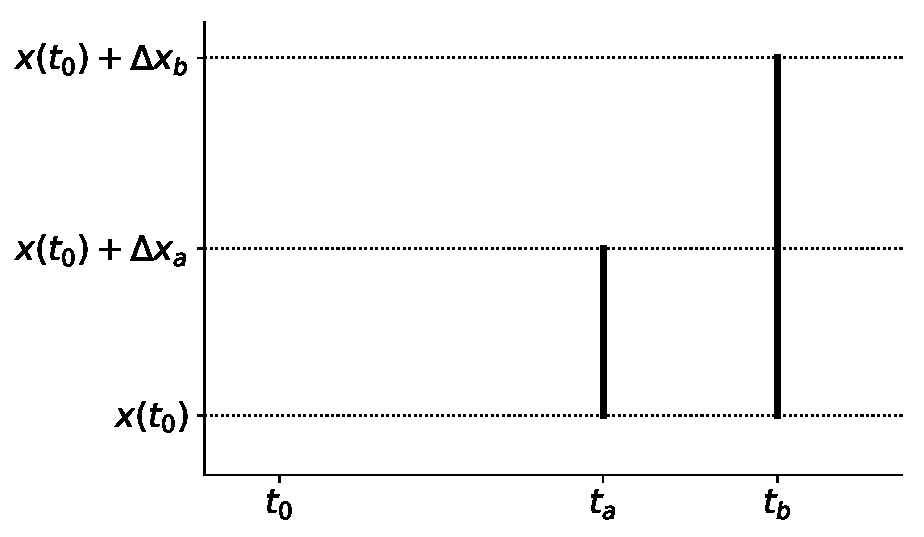
\includegraphics[width=0.7\textwidth]{./figures/setup.pdf}
\caption{
The basic setup of the model. A decision maker faces a choice at time $t_0$ between option $a$, which guarantees a payoff of $\Dx_a$ at time $t_a$, and option $b$, which guarantees a payoff of $\Dx_b>\Dx_a$ at time $t_b>t_a$.
}
\flabel{basicsetup}
\end{figure}

This setup corresponds to a standard question that arises in the context of temporal discounting, \eg ``would you prefer to receive \$100 tomorrow or \$200 in a month's time?'' Despite its apparent simplicity, answering this question requires additional assumptions. Or, put another way, the problem is underspecified. One extra assumption needed concerns the dynamics under which the decision-maker's wealth grows. Often it is assumed that wealth grows exponentially, compounding continuously at a constant riskless rate like funds in a savings account. Another assumption concerns the time frame of the decision, specifically whether a decision-maker accepting the earlier payoff at $t_a$ is free immediately to make his next decision, or whether he must wait until the later time $t_b$ (or, indeed, some other time) before the decision can be repeated. Such assumptions are needed to compute decision-maker's maximand -- the growth rate of his wealth -- so that the options can be compared quantitatively.
%XXXOP or over some other $\Delta t$? As $\Delta t \to \infty$ all growth rates go to zero, and our framework becomes degenerate (it can't select an optimum). This could be interpreted as the one-shot setup.XXX

We will describe four different specifications of this basic setup. In each we will calculate the growth rates, $g_a$ and $g_b$, of wealth associated with options $a$ and $b$. The decision maker prefers the option whose growth rate is larger.

We will also infer the discount factor (\textit{DF}) from this analysis. This is the multiplicative factor, $\delta$, by which the later payoff, $\Dx_b$, must be multiplied to equal the earlier payoff, $\Dx_a$, when the payoff amounts and times are such that the decision maker is indifferent between the two options ($\left(t_a,\Dx_a\right) \sim \left(t_b,\Dx_b\right)$). In symbols,

\be
\delta \equiv \left.\frac{\Dx_a}{\Dx_b}\right|_{g_a=g_b},
\ee
\ie the ratio of payoffs under the constraint that the growth rates of wealth are equal.
%To calculate to DF, we evaluate the ratio between the payoff $\Dx_a$ and the payoff $\Dx_b$ under the assumption that the the growth rates $g_a$ and $g_b$ are equal.

As we show below, this setup predicts decisions equivalent to hyperbolic and exponential discounting under different specifications. Some specifications of the model predict preference reversal.
%Our model differs from many standard models in the literature by assuming that decision makers maximize the growth rate of their wealth, rather than the expected change in their utility.
%It has been shown to be equivalent in some cases, under specific dynamics and specific utility function choices~\citep{peters2018time}. It is further discussed in~\Sref{discussion}.

\section{Results}\label{sec:results}

\subsection{Specification}

We begin by describing four different specifications for our basic setup. Each specifies two aspects necessary to quantify the growth rate of wealth: the time frame of the decision; and the dynamics under which wealth evolves.

The time frame is a key aspect, often left unspecified in similar setups in the literature. Consider the following scenarios:

\begin{enumerate}
    \item Dana, the real estate developer, loves to work and always wants to keep busy with her building projects, she always gets paid at their completion. Dana has a choice between a project that lasts three months and a project that lasts six months. 
    \item Every year, Nate the Naval officer must go for either a three month long mission or a six month long mission. He is given the choice at the beginning of every year (both missions finish before the end of the year). He is paid right after his mission is completed.
\end{enumerate}

In the first scenario, the time frame depends on the choice made. We call this the \textit{elastic} time frame because Dana is more flexible to pursue other opportunities if she chooses the shorter project. On the other hand, if she chooses the longer project, it locks her in a for a longer time period, which means it also changes when she will have another choice.  

In the second scenario, the important element to note is that no matter which choice is made, it will not affect the timing of future choices. Said otherwise, the time frame is independent of the choice, so we say it is \textit{fixed}.
%That is, the timing of Nate's next choice is not affected by his decision. 

In our model, we must choose the time period over which the growth rates of wealth in each option are computed. We can choose it to be the time period associated with each payoff, \ie $t_a-t_0$ for option $a$ and $t_b-t_0$ for option $b$. This specification corresponds to Dana's situation, the elastic time frame specification. Or we can choose it always to be the longer time period, $t_b-t_0$, resembling Nate's dilemma, the fixed time specification.

%For convenience, we denote the two periods between the decision time and the known future payoff times as $\Dt_a \equiv t_a-t_0$ and $\Dt_b \equiv t_b-t_0$. Additionally, we denote the known delay between the two payoffs as $D \equiv t_b-t_a$.


%\textcolor{red}{\begin{enumerate}
%    \item A builder must choose between two jobs starting tomorrow, one paying \$1,000 for a week's work and the other paying \$3,000 for a month's work, with both sums being paid on completion of the work.
%    \item An author must choose %between receiving \$30,000 in advance or \$50,000 on production of a book that will take a year to write.
%\end{enumerate}}

% \textcolor{red}{In the first scenario, the time frame depends on the choice made: one week for the smaller job; one month for the larger job. If the builder chooses the smaller job, he is free to pursue other opportunities during the three-and-a-bit weeks between its completion and the completion of the larger job. But if he chooses the larger job, he can do nothing else for the whole month. Although the guaranteed payoff is greater, the larger job has an opportunity cost relative to the smaller one.}

%\textcolor{red}{In the second scenario, the time frame is independent of the choice: in both cases, the author must work for one year. In particular, taking the earlier payoff does not allow her (ethically, at least) to pursue other opportunities during the period between it and the later payoff that she declined.}


%\textcolor{red}{In our model, we must choose the time frame over which the growth rates of wealth in each option are computed. We can choose it to be the time period associated with each payoff, \ie $\Dt_a$ for option $a$ and $\Dt_b$ for option $b$. This specification reminds us of the builder's choice and we will call it the elastic time frame specification. Or we can choose it always to be the longer time period, $\Dt_b$, resembling the author's dilemma. We will call this the fixed time frame specification.}

%One possibility is to assume a fixed time frame -- the decision maker faces the choice every $\Dt_b$. In this case, in order to compare between the two choices, we will evaluate the growth rates between $t_0$ and $\Dt_b$ in both options. Another possible specification of time frame, is that the decision maker faces a choice after the payoff is exercised, \ie after $\Dt_a$ if option $a$ was chosen and after $\Dt_b$ if option $b$ was chosen. In this case, we will evaluate the growth rate for option $a$ at time $\Dt_a$, and for option $b$ at $\Dt_b$. The former time frame will be labeled the fixed time frame and the latter the elastic time frame.

As described in~\Sref{model}, the wealth dynamics can also take different forms, and we will address two specific common cases: additive and multiplicative wealth dynamics. We note that under the multiplicative dynamics it is assumed that the payoff itself is re-invested at the risk-free rate. For additive dynamics there is essentially no re-investment of the payoff -- income in this dynamic is independent of wealth.

We will discuss the four specifications, as illustrated in~\fref{tree}. In each case we will: compute the growth rates $g_a$ and $g_b$ associated with each option; compare them to determine the conditions under which each option is preferred; elicit the form of temporal discounting equivalent to our decision model; and, finally, determine whether PR is predicted.

\begin{figure}[!htb]
\centering
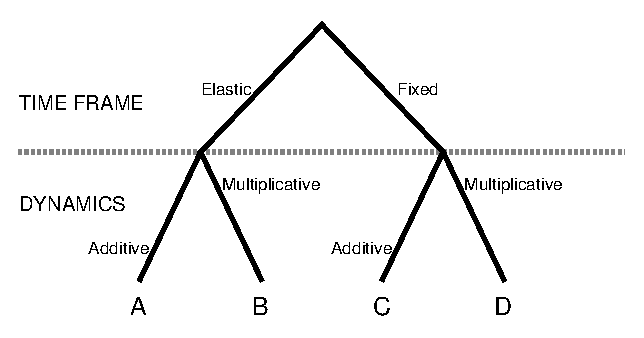
\includegraphics[width=0.7\textwidth]{./figures/tree.eps}
\caption{The four model specifications, determined by specifying a time frame and wealth dynamics. The labels A, B, C, and D, are used for the different cases.}
\flabel{tree}
\end{figure}

\subsection{Case A -- Elastic time frame with additive dynamics}\label{sec:case_A}

Specification: the period for computing the growth rate is that between the decision and the chosen payoff; and the wealth dynamics are additive, with growth rate $k$.

We begin by writing down the final wealth under the two options, evaluated at $t_a$ and $t_b$ respectively:
\bea
x_a\left(t_a\right) &=& x\left(t_0\right) + \Dx_a + k(t_a-t_0)\,;\\
x_b\left(t_b\right) &=& x\left(t_0\right) + \Dx_b + k(t_b-t_0)\,.
\eea

The growth rates are:
\bea
g_a &=& \frac{x_a\left(t_a\right) - x\left(t_0\right)}{t_a-t_0} = \frac{\Dx_a}{t_a-t_0} + k\,;\\
g_b &=& \frac{x_b\left(t_b\right) - x\left(t_0\right)}{t_b-t_0} = \frac{\Dx_b}{t_b-t_0} + k\,.
\eea

It follows that the criterion $g_a > g_b$ is
\be
\frac{\Dx_a}{t_a-t_0} > \frac{\Dx_b}{t_b-t_0}\,.
\ee

This criterion suggests that, under this specification, the only thing that matters to the decision maker is the linear payoff rate of each option.

If we treat the payoff amounts, $\Dx_a$ and $\Dx_b$, and payoff times, $t_a$ and $t_b$, as fixed parameters of the problem, then we can elicit the dependence of the decision on the decision time, $t_0$. When the payoffs are far ahead in the future, the ratio of the growth rates approaches $\lim_{t_0\to-\infty}\frac{g_a}{g_b}=\frac{\Dx_a}{\Dx_b}$, and $g_a<g_b$ since we have assumed $\Dx_a<\Dx_b$. When the earlier payoff is imminent, \ie as $t_0\to t_a$, $g_a$ grows without bound while $g_b$ remains finite and so $g_a>g_b$. In other words, as time passes, our decision model under this specification predicts preference reversal from the later, larger payoff to the earlier, smaller payoff. This is illustrated in~\fref{caseA}.

\begin{figure}[!htb]
\centering
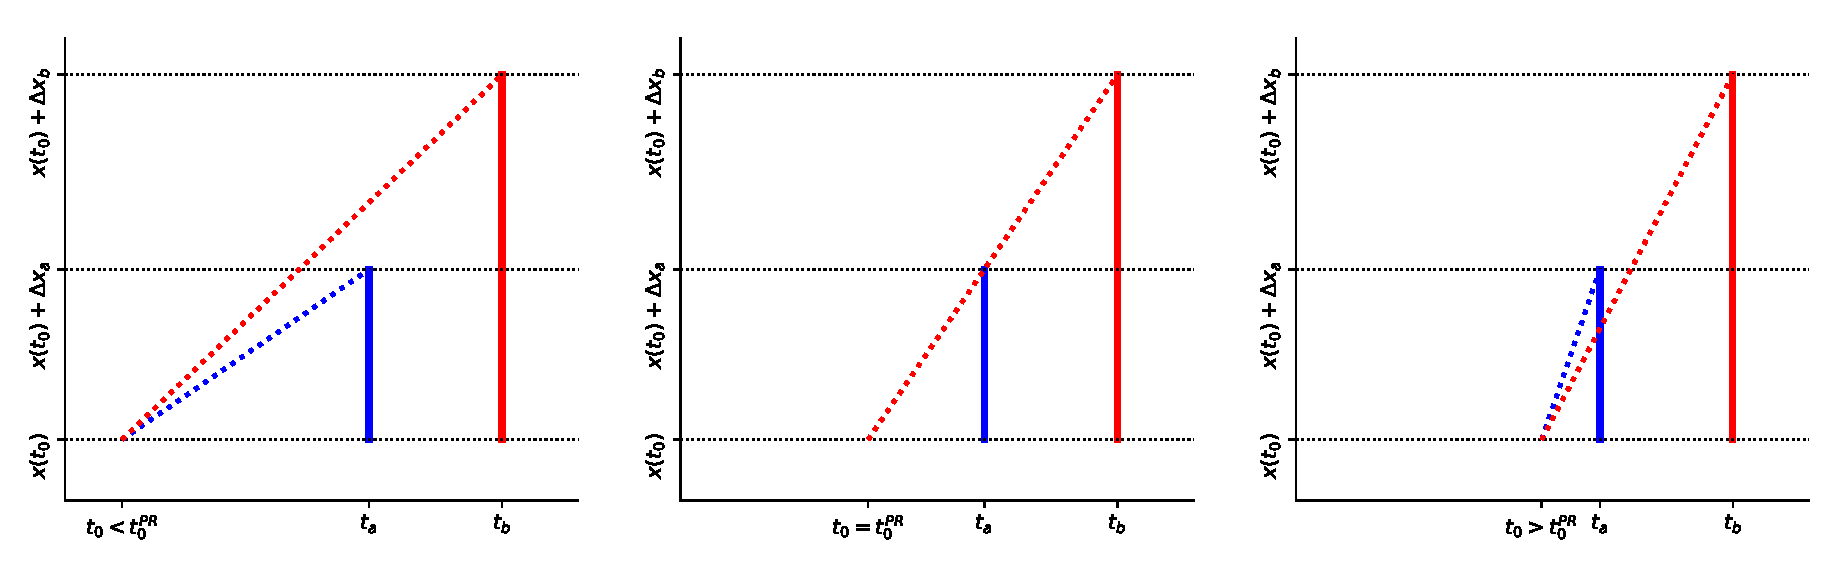
\includegraphics[width=1.0\textwidth]{./figures/reversals.eps}
\caption{Preference reversal in case A. From left to right panel, $t_0$ increases, that is, the time of the payoffs approaches, while all other parameters are unchanged. Initially, option $b$ is preferable, having the higher growth rate. At a later time $t_0=t_0^{PR}$, given by~\eref{t0PR}, both options imply equal growth, and preference reversal occurs. At later times option $a$ is preferable.}
\flabel{caseA}
\end{figure}

%\begin{figure}
%\centering
%\begin{picture}(420,100)(0,0)
%\put(-50,0){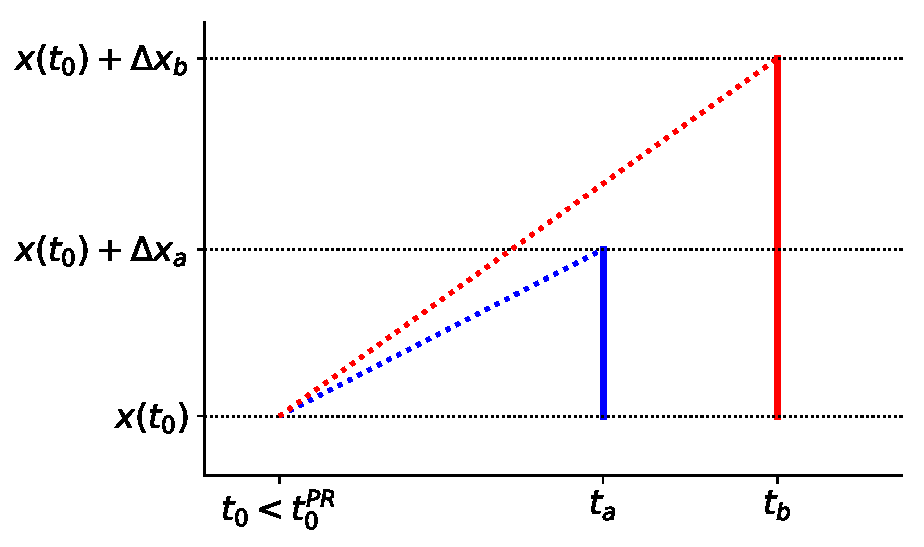
\includegraphics[width=0.39\textwidth]{./figures/reversal_1.pdf}}
%\put(110,0){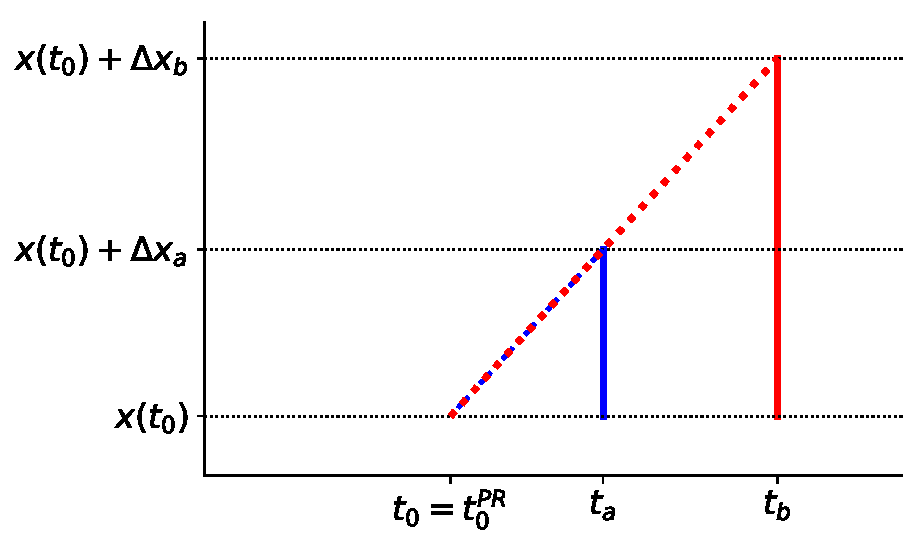
\includegraphics[width=0.39\textwidth]{./figures/reversal_2.pdf}}
%\put(270,0){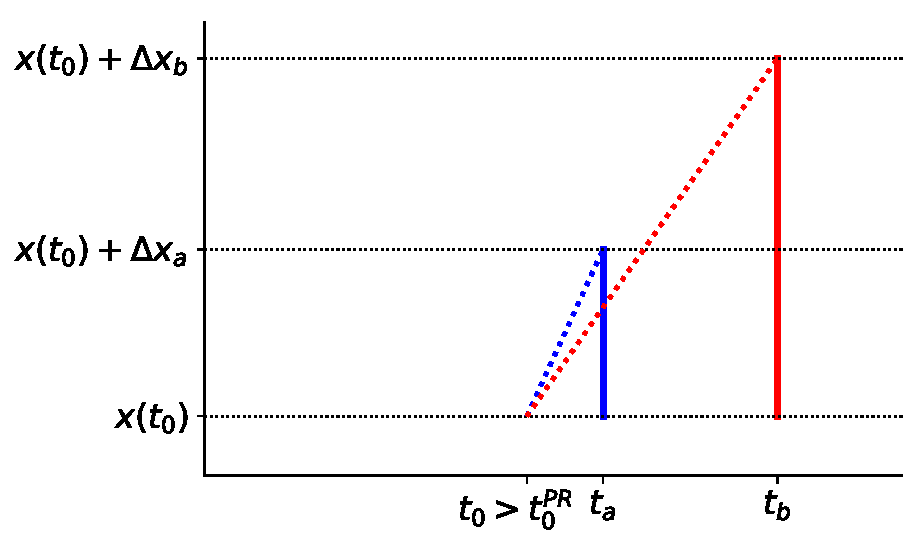
\includegraphics[width=0.39\textwidth]{./figures/reversal_3.pdf}}
%\end{picture}
%\caption{
%Preference reversal in case A. From left to right panel, $t_0$ increases, that is, the time of the payoffs approaches, while all other parameters are unchanged. Initially, option $b$ is preferable, having the higher growth rate. At a later time $t_0=t_0^{PR}$, given by \eref{t0PR}, both options imply equal growth, and preference reversal occurs. At later times option $a$ is preferable. 
%}
%\flabel{caseA}
%\end{figure}

%It shows that the payoff rate of option $b$ is higher than that of option $a$, which makes it preferable. This holds for some time. However, at some point in time, this changes and the payoff rate of option $a$ would be higher. Assuming that initially option $g_b > g_a$, there will always be a point in time in which PR will occur. If time $\tau$ elapsed from $t_0$, than the updated payoff rates of options $a$ and $b$ are $\frac{\Dx_a}{\Dt_a - \tau}$ and $\frac{\Dx_b}{\Dt_b - \tau}$, respectively. The reversal will occur when these are equal, or
%\be
%\tau_{\text{reversal}} = \frac{\Dt_a\Dx_b - \Dt_b\Dx_a}{\Dx_b - \Dx_a}\,.
%\ee

We can compute the decision time, $t_0^\text{PR}$, at which preference reversal occurs by setting $g_a=g_b$ to give
\be
t_0^\text{PR} = \frac{\Dx_b t_a - \Dx_a t_b}{\Dx_b - \Dx_a}.
\elabel{t0PR}
\ee

We can also find the effective discount factor under this specification. When $g_a=g_b$, we have
\be
\delta = \frac{\Dx_a}{\Dx_b} = \frac{t_a-t_0}{t_b-t_0} = \frac{1}{1+\frac{t_b-t_a}{t_a-t_0}},
\ee
where we have made the final manipulation to express $\delta$ in hyperbolic form. We see that the discount factor depends on two time periods: that between decision and the earlier payoff, $t_a-t_0$, which we will call the \textit{horizon}; and that between the two payoffs, $t_b-t_a$, which we which we will call the \textit{delay}.\footnote{Indeed, the problem is fully specified by these two time periods and the two payoff amounts. The actual times, $t_0$, $t_a$, $t_b$, are not needed to specify the problem because, when computing growth rates, only elapsed times matter. The time origin is arbitrary.} If we define $\hor\equiv t_a-t_0$ and $\del\equiv t_b-t_a$, we can write the discount factor as
\be
\delta = \frac{1}{1+\del/\hor},
\ee
which is expressed in the conventional way as a hyperbolic function of the delay, $\del$. The psychological degree of discounting parameter used in mainstream models is replaced here by $1/\hor$, the reciprocal of the horizon. As the horizon gets shorter, $1/\hor$ becomes larger, $\delta$ gets smaller, and the later payoff becomes less favorable. No knowledge of the decision-maker's psychology is required in this setup -- only the postulate that she prefers her wealth to grow faster rather than slower.

%The discount factor, $\delta$, is the factor by which the later payoff, $\Dx_b$, must be multiplied to equal the earlier payoff, $\Dx_a$, under indifference between options $a$ and $b$. Practically, it can be found by considering the equality of growth rates $g_a$ and $g_b$, which is the condition for indifference. $\delta$ is typically presented as a function of the time difference between options. In our setup this would be $\Epsilon \equiv \Dt_b - \Dt_a$.
%
%\textcolor{red}{
%Now that we have the hyperbolic DF in terms of the delay, $\Dt_b-\Dt_a$, and the time to the first payoff, $\Dt_a$, as
%\be
%\delta = \frac{1}{1+\frac{\Dt_b-\Dt_a}{\Dt_a}} = \frac{1}{1+kD},
%\ee
%it would be much clearer to present PR as a consequence of changing the time to the first payoff rather than the reference time. Then $t_0\to t_0+\Dt_a$ is simply $\Dt_a\to0$, which is also expressible as $k\to\infty$. This minor reframing will require some changes below, including to the figure, because we would treat $t_0$ as fixed and $\Dt_a$ as movable.
%}
%\textcolor{red}{
%Do we need $\Epsilon$? The letter has no intuitive meaning (to me) and perhaps we can get away without relabelling $\Dt_b-\Dt_a$. If not, $D$ for delay or $W$ for wait might be better.
%}
%XXXOP: not sure -- I like the physical time $t_0$ changing. What happens in real life is that time ticks on and we get swept towards $t_a$, it's not that we sit still in time, and someone tunes $t_a$. Agree about $\Epsilon$ -- better letter?XXX
%
%
%In case A we therefore get
%\be
%\delta_A = \frac{\Dx_a}{\Dx_b} = \frac{\Dt_a}{\Dt_b} = \frac{1}{1+\frac{1}{\Dt_a} \Epsilon}\,.
%\ee
%
%This is exactly hyperbolic discounting with degree of discounting $\kappa = \frac{1}{\Dt_a}$.

Finally, we note that the background growth rate, $k$, of the decision-maker's wealth does not appear in the decision criterion. This is because wealth growth under additive dynamics is not affected by exogenous cash flows: the gain $k\Dt$ over period $\Dt$ occurs regardless of other payoffs received. This contrasts with multiplicative dynamics, where payoffs can be subjected to the growth process through re-investment.

\subsection{Case B -- Elastic time frame with multiplicative dynamics}\label{sec:case_B}

Specification: the time frame for computing the growth rate is time to the chosen payoff; and the wealth dynamics are multiplicative, with growth rate $r$.

We follow the same steps as in case A. Wealth evolves to:
\bea
x_a\left(t_a\right) &=& x\left(t_0\right) e^{r(t_a-t_0)} + \Dx_a\,;\\
x_b\left(t_b\right) &=& x\left(t_0\right) e^{r(t_b-t_0)} + \Dx_b\,.
\eea

The corresponding growth rates are:
\bea
g_a &= \frac{1}{t_a-t_0} \log{\left(\frac{x_a\left(t_a\right)}{x\left(t_0\right)}\right)} = \frac{1}{t_a-t_0}\log{\left(1 + \frac{\Dx_a}{x\left(t_0\right)e^{r(t_a-t_0)}}\right)} + r \elabel{ga_B}\\
g_b &= \frac{1}{t_b-t_0} \log{\left(\frac{x_b\left(t_b\right)}{x\left(t_0\right)}\right)} = \frac{1}{t_b-t_0}\log{\left(1 + \frac{\Dx_b}{x\left(t_0\right)e^{r(t_b-t_0)}}\right)} + r\,.\elabel{gb_B}
\eea

This setting displays preference reversal: $g_a<g_b$ for $t_0$ sufficiently far away from $t_a$ (long horizon); and $g_a>g_b$ for $t_0$ sufficiently close to $t_a$ (short horizon). No closed-form expression for the reversal time, $t_0^\text{PR}$, is available.

Similarly, the discount factor $\delta$ cannot be derived explicitly. However, if we assume small payoffs relative to wealth, \ie $\Dx_a \ll x\left(t_0\right)e^{r(t_a-t_0)}$ and $\Dx_b \ll x\left(t_0\right)e^{r(t_b-t_0)}$, then, setting $g_a=g_b$ and using the first-order approximation $\log(1+\epsilon)\approx\epsilon$ for $\epsilon\ll1$, we get
\be
\delta = \frac{\Dx_a}{\Dx_b} \approx \frac{(t_a-t_0)e^{r(t_a-t_0)}}{(t_b-t_0)e^{r(t_b-t_0)}} =
\frac{e^{r(t_a-t_b)}}{1+\frac{t_b-t_a}{t_a-t_0}}\,.
\ee
Using the previous definitions of $\hor$ and $\del$, we can write this as
\be
\delta \approx \frac{e^{-r\del}}{1+\del/\hor}\,,
\ee
which is a hybrid of hyperbolic and exponential discounting. We note again that only the elapsed times, $\hor$ and $\del$, appear in the discount factor. However, that the background wealth growth rate, $r$, no longer cancels out when dynamics are multiplicative, as does $k$ when they are additive.

Case B also displays another type of preference reversal. Varying initial wealth $x(t_0)$ while keeping all other parameters fixed can lead to a switch from $g_a>g_b$ to $g_a<g_b$, as illustrated in~\fref{reversal_B}.
%An example is given in panel A of \fref{reversal_2}, and 

\begin{figure}[!htb]
\centering
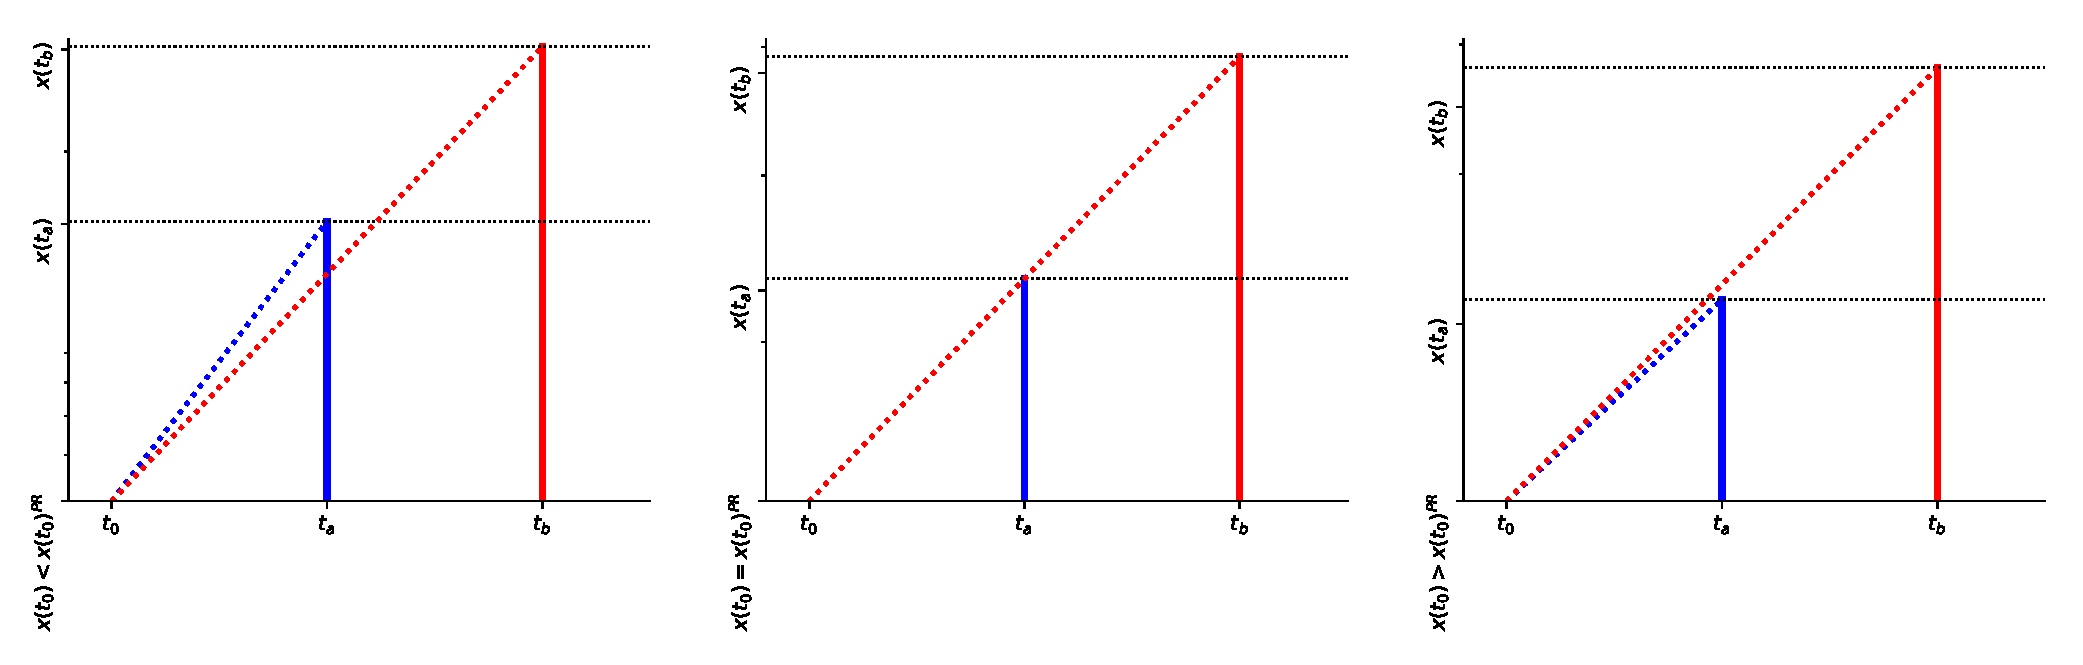
\includegraphics[width=1.0\textwidth]{./figures/reversals_B.eps}
\caption{Preference reversal in response to wealth changes, in case B, logarithmic vertical scales. Initial wealth $x(t_0)$ increases from left to right panel (\$500, \$2277, \$5,000), while all other parameters are unchanged ($t_0=$ today, $t_a=1$~year from today, $t_b=2$~years from today, $\Dx_a=\$1000$, $\Dx_b=\$2500$, $r=0.03$~per annum). At low wealth, option $a$ is preferable, having the higher growth rate, according to~\eref{ga_B} and~\eref{gb_B}. At a greater wealth, $x(t_0)^{PR}\approx \$2277$, both options imply equal growth, and preference reversal occurs. At even greater wealth, option $b$ is preferable: the poor behave optimally by choosing the small early payoff.}
\flabel{reversal_B}
\end{figure}

%\begin{figure}
%\centering
%\begin{picture}(420,100)(0,0)
%\put(-50,0){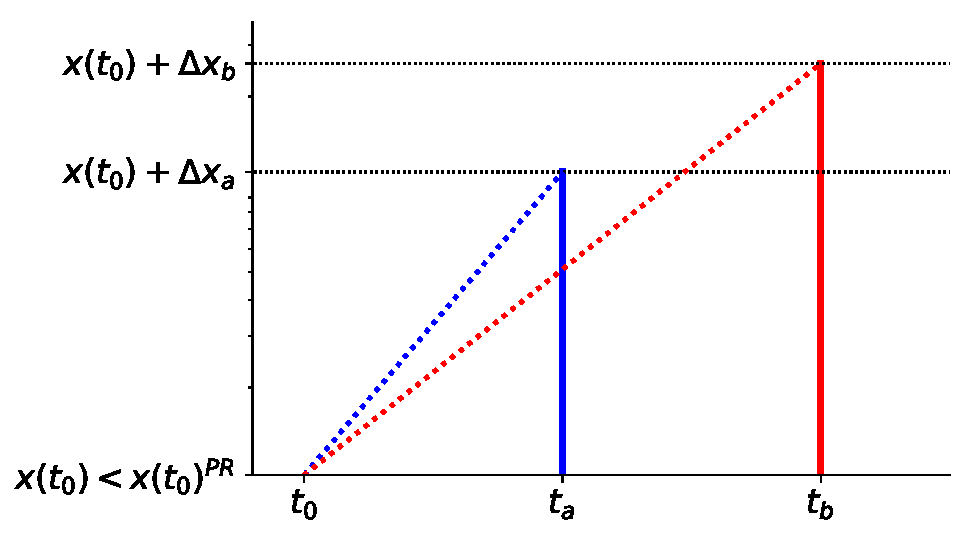
\includegraphics[width=0.39\textwidth]{./figures/reversal_B_1.pdf}}
%\put(110,0){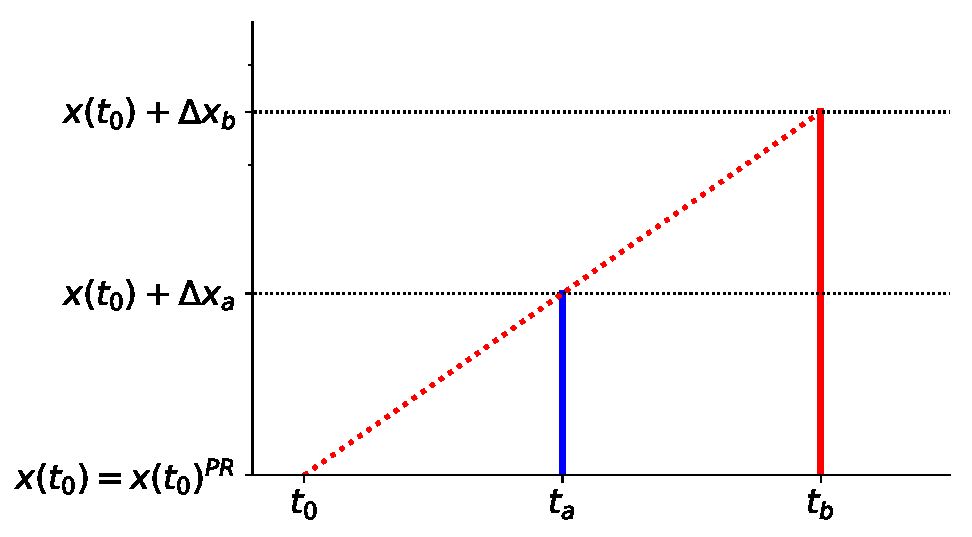
\includegraphics[width=0.39\textwidth]{./figures/reversal_B_2.pdf}}
%\put(270,0){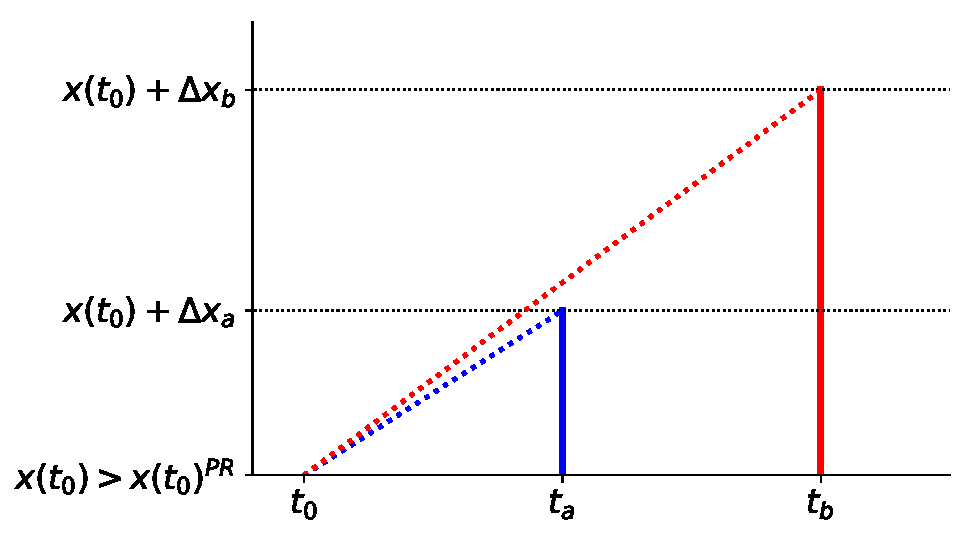
\includegraphics[width=0.39\textwidth]{./figures/reversal_B_3.pdf}}
%\end{picture}
%\caption{
%Preference reversal in response to wealth changes, in case B, logarithmic vertical scales. Initial wealth $x(t_0)$ increases from left to right panel (\$500, \$2277, \$5,000), while all other parameters are unchanged ($t_0=$ today, $t_a=1$~year from today, $t_b=2$~years from today, $\Dx_a=\$1000$, $\Dx_b=\$2500$, $r=0.03$~per annum). At low wealth, option $a$ is preferable, having the higher growth rate, according to \eref{ga_B} and \eref{gb_B}. At a greater wealth, $x(t_0)^{PR}\approx \$2277$, both options imply equal growth, and preference reversal occurs. At even greater wealth, option $b$ is preferable: the poor behave optimally by choosing the small early payoff.
%}
%\flabel{reversal_B}
%\end{figure}

The difference $g_a-g_b$, from~\eref{ga_B} and~\eref{gb_B}, is shown as a function of $x(t_0)$ in~\fref{reversal_B2}. This type of preference reversal can be expressed as follows: under certain circumstances, it is growth-optimal for people of lower wealth to choose a small early payoff, whereas it is growth-optimal for wealthier individuals to hold out until the later larger payoff. This predicts the findings of~\citet{epper2018time}, that ``individuals with relatively low time discounting are consistently positioned higher in the wealth distribution''.

\begin{figure}[!htb]
\centering
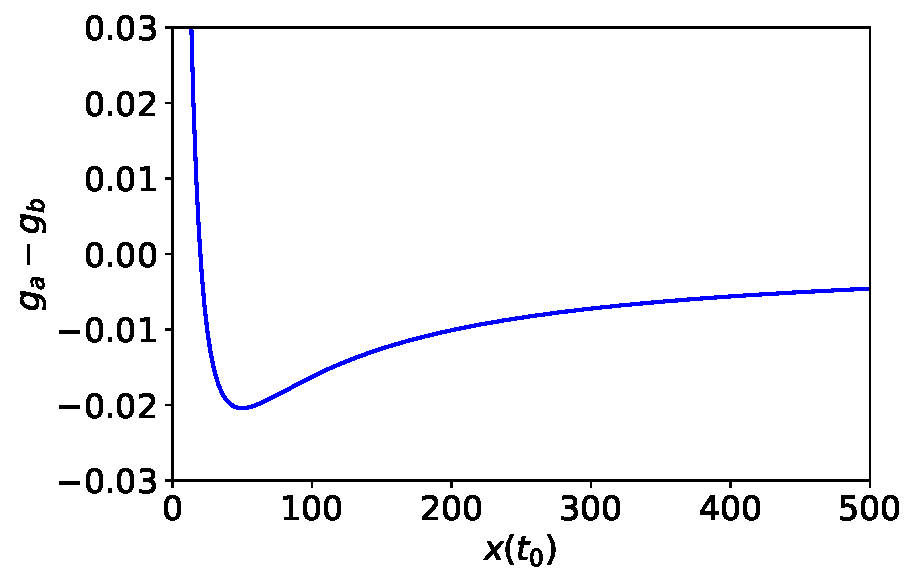
\includegraphics[width=0.7\textwidth]{./figures/ga_gb.pdf}
\caption{The difference $g_a-g_b$ is positive when the earlier payoff is preferable, and otherwise negative. We see that for small initial wealths $x(t_0)$ the earlier smaller payoff is preferred, whereas for large initial wealth the later larger payoff is preferred (parameters as in~\fref{reversal_B}).}
\flabel{reversal_B2}
\end{figure}

\FloatBarrier
\subsection{Case C -- Fixed time frame with additive dynamics}\label{sec:case_C}

Now we assume additive dynamics as in case A, but with a fixed time frame so that the outcomes of both choices are compared at $t_b$. The wealths evolve to: \bea
x_a\left(t_b\right) &=& x\left(t_0\right) + \Dx_a + k(t_b-t_0)\,; \\
x_b\left(t_b\right) &=& x\left(t_0\right) + \Dx_b + k(t_b-t_0)\,.
\eea
The growth rates are:
\bea
g_a &=& \frac{x_a\left(t_b\right) - x\left(t_0\right)}{t_b-t_0} = \frac{\Dx_a}{t_b-t_0} + k\,;\\
g_b &=& \frac{x_b\left(t_b\right) - x\left(t_0\right)}{t_b-t_0} = \frac{\Dx_b}{t_b-t_0} + k\,.
\eea
Note that the wealth and its growth rate under option $b$ are the same as in case A, since they were already evaluated at $t_b$ there.

Since we have assumed $\Dx_b > \Dx_a$, option $b$ is always preferred to option $a$. This is a trivial case -- if we assume additive wealth dynamics and comparing the growth rates at the same time (or assuming repetition over fixed periods), then the only thing that matters to the decision-maker is payoff size. In this case, the discount factor $\delta$ cannot be defined, since the later, larger payoff is always preferred and the indifference condition is never satisfied.

\subsection{Case D -- Fixed time frame with multiplicative dynamics}\label{sec:case_D}

Finally, we assume multiplicative dynamics and a fixed time frame. This is the specification that corresponds to the standard assumptions usually considered in temporal discounting -- that wealth is continuously compounding at the risk-free rate and that payoffs are re-invested at this rate.

The chief difference from case B is that the earlier payoff, $\Dx_a$, if chosen, is treated as growing exponentially from $t_a$ to $t_b$. The wealths evolve from $t_0$ to $t_b$ as follows:
\bea
x_a\left(t_b\right) &=& x\left(t_0\right) e^{r(t_b-t_0)} + \Dx_a e^{r(t_b-t_a)}\,;\\
x_b\left(t_b\right) &=& x\left(t_0\right) e^{r(t_b-t_0)} + \Dx_b\,.
\eea
The corresponding growth rates are:
\bea
g_a &= \frac{1}{t_a-t_0} \log{\left(\frac{x_a\left(t_a\right)}{x\left(t_0\right)}\right)} = \frac{1}{t_b-t_0}\log{\left(1 + \frac{\Dx_a e^{r(t_b-t_a)}}{x\left(t_0\right)e^{r(t_b-t_0)}}\right)} + r\\
g_b &= \frac{1}{t_b-t_0} \log{\left(\frac{x_b\left(t_b\right)}{x\left(t_0\right)}\right)} = \frac{1}{t_b-t_0}\log{\left(1 + \frac{\Dx_b}{x\left(t_0\right)e^{r(t_b-t_0)}}\right)} + r\,.
\eea
Note that the evolution of wealth under option $b$ is the same as in case B.


The criterion $g_a > g_b$ is actually very simple, since only the second term in the logarithm is different and so only this must be compared. Thus, $g_a > g_b$ if
\be
\Dx_a e^{r(t_b-t_a)} > \Dx_b\,,
\ee
or, in terms of the delay, if
\be
\Dx_a e^{r\del} > \Dx_b\,.
\ee

The discount factor is similarly expressed by setting the growth rates to be equal. Then we get $\Dx_a e^{r\del} = \Dx_b$ and
\be
\delta = \frac{\Dx_a}{\Dx_b} = e^{-r\del}\,,
\ee
which is the standard exponential discounting result. The interpretation is straightforward: if it is possible to re-invest the earlier payoff such that, by the time of the later payoff, it will exceed the later payoff amount, then option $a$ is preferable to option $b$ (and \textit{vice versa}). Note that, with this specification, the horizon is irrelevant. All that matters is the payoff amount after possible re-investment.

\section{Discussion}\label{sec:discussion}

This paper describes a model in which a decision maker chooses between two certain payoffs realized at different, certain points in time. We assume that a decision is made by comparing the growth rate of wealth associated with each option. We then study temporal discounting in a deterministic setting. In this setting the model is consistent with the standard von Neumann-Morgenstern axioms.

The main finding is that discounting can be interpreted as growth rate optimization. We find that depending on the wealth dynamics assumed by the decision maker, growth rate optimization can be equivalent to hyperbolic discounting. It then predicts preference reversal. It can also be equivalent to a mixed case of hyperbolic and exponential discounting, which also implies preference reversal. Under multiplicative dynamics, we find that growth rate optimization reproduces standard exponential discounting. This reveals the standard form of discounting as one of many possible forms of discounting, each of which is optimal under a different type of wealth growth.

The model predicts another type of reversal under multiplicative dynamics. It can be growth-optimal for people of lower wealth to choose a small early payoff, whereas it is growth-optimal for wealthier individuals to hold out until the later larger payoff. This is inline with the experimental and empirical findings of~\citet{epper2018time}, that ``individuals with relatively low time discounting are consistently positioned higher in the wealth distribution''.

We emphasize that no knowledge of the decision-maker's psychology is required in our setup -- only the postulate that she prefers her wealth to grow faster rather than slower. This postulate is enough for to predicting a decision maker's discount rates used in mainstream models. Yet, we also note that this paper discusses discounting from a theoretical perspective. An important complementary step of this research would be comparing the theoretical predictions of the results to empirical and experimental results. In particular, the predicted discount factors and discount rates can be compared to results from controlled experiments. This is planned for future work.

%A fundamental question about the model is why would someone maximize growth instead of expectation value of utility? This, of course, differs from the traditional framework for analyzing decisions in economics, usually taking it as axiomatic that people maximize utility. Yet, this is only one way of studying optimal choice under different conditions. At the same time it is important to note that without risk, the choice axiom used in this paper, 
%it is important to question where does the utility optimizing mechanism come from?

%The framework we used here has an answer -- evolutionary mechanisms. That is, as time passes some utility functions dominate over others. The utility functions that do so over the long run are growth-optimal. Technically, they are ergodicity mappings: maximizing the expected value of such a utility function is guaranteed to maximize wealth over time.

%An additional extension is the inclusion of risk. The standard explanations to hyperbolic discounting consist of a behavioral response to risk~\citep{sozou1998hyperbolic,dasgupta2005uncertainty}, while here we showed that hyperbolic discounting can be observed even in the absence of uncertainties in the payoffs or in their timing. Adding uncertainty to our model might create additional forms of temporal discounting, which might be more realistic and closer to empirical evidence.
%XXXOP: we have already done the random case. That's what we usually do. Ergodic growth rate optimization includes randomness, it's just interesting that even without randomness, i.e. just discounting, we also recover a lot of known results.


%\textcolor{green}{Given the framework here, risk can be interpreted in two ways. Either it represents the actual probability of an arrival of a choice or it represents the belief about the environment. The corresponding discount rate then be some weighted average between the discount rates presented here. }

%Though utility functions are traditionally used for individuals, this framework implies that even firms should have utility functions. That is, why should firms discount hyperbolically? If a firm has a fixed staff and cannot undertake numerous projects at the same time and has access to some interest rate, then it should discount hyperbolically. If the evolutionary mechanism is considered, maximizing the expected value can actually be considered as merely a case of bounded rationality. The process of updating beliefs based solely on observation without reference to the environment, may be ecologically irrational.

%Whether actual decision makers behave this way is an empirical question, nevertheless this theory relative to the classic case, has more Popperian content inscribed in it. So we consider that this framework offers a rich agenda for research. Yet, the empirical implications of the model do have falsifiable content. That is, after we observe a specific discount factor from someone, we can deduce the environment they are in. For instance, if someone is in a changing environment, we should expect them use the ensemble average. If, on the other hand, the environment is constant then we predict that they will behave more like the time average. An objective measure of opportunity could be one way to construct such a measure.

%This is only one way to interpret the model. Another way would be that the preferences which are revealed, also reveal a belief set. However, this case is not as empirically interesting because the belief set is defined by the preferences and does not imply a cognitive awareness of the implied belief. That is, just because a set of beliefs are implied, this does not mean that they can be solicited. Why might we not be able to solicit preferences? For it to be possible to solicit preferences it must assumed that the decision rule used in experiments is the same as the one used in the real world. Well how do we verify that the actual preferences are the same ones as the ones that were solicited? By looking to see consistency between solicitation and the real world. 

%It is possible to find that agents make use of a specific decision rule only for such experiments. We then should ask why do some people change their decision rules when solicited whilst others do not? Ultimately, this question must be answered without looking at solicited preferences. So there is still a need to look at the environment of the agent. Focusing on beliefs does not in fact ever yield satisfactory answers because the meta question will always exist.

%Using solicited preferences does in fact requires going back to the real world in any case, so it can be skipped altogether. The approach in this paper differs by offering the potential to omit the solicitation. Observing data on how decision makers make investment choices in the real world, can describe the discount rate. If we cannot tell which specification of the model should be used, more information may be used. For instance, if someone has access to a good investment manager or if they often have investment opportunities. The advantage of this approach is to bypass the need to look at verbally stated beliefs.

\newpage

\bibliography{discountingbib}


\clearpage

\appendix

%\section{Relative mobility measures independence}
%\label{app:app0}

\section{Proofs}
\label{app:appA}

\subsection{Proof of \preflong{trans}}

We assume three tuples $A\equiv\left(t_a,\Dx_a\right)$, $B\equiv\left(t_b,\Dx_b\right)$ and $C\equiv\left(t_c,\Dx_c\right)$, where $t_a < t_b < t_c$. Given time $t_0$ ($< t_a$) and an initial wealth $x\left(t_0\right)$, the vectors $\{t_0,x\left(t_0\right),t_a,\Dx_a,t_b,\Dx_b\}$ and $\{t_0,x\left(t_0\right),t_b,\Dx_b,t_c,\Dx_c\}$ are both CIPPs.

If $A \prec B$ and $B \prec C$ then $g_a < g_b$ and $g_b < g_c$. Also $t_a < t_b < t_c$. Therefore $\{t_0,x\left(t_0\right),t_a,\Dx_a,t_c,\Dx_c\}$ is a CIPP and $g_a < g_c$, so $A \prec C$.

\qed
\end{document}